%!TEX root = thesis.tex

\chapter{Implementation}
\label{chap:impl}

Implementation of the methods are described in this chapter.

\section{Preparing linked data}
Linked data has been prepared that is used to retrieve and process sensor data on the semantic web (Figure \ref*{fig:Static}). This is done for vector data sets of administrative units and land cover features, and for raster data sets of \ac{eea} grids with a resolution of 10km\textsuperscript{2} and 100km\textsuperscript{2}. 

\begin{figure}
	%\centering
	\includegraphics[width=0.7\linewidth]{UML/staticdata2.PNG}
	\caption{Model of vector and raster features}
	\label{fig:Static}
\end{figure}


Three types of administrative units have been converted to linked data: countries, provinces and municipalities. Every administrative unit has a name, `type' and (multi)polygon geometry assigned to it (Figure \ref{fig:Static}). The administrative unit type is defined by DBPedia \ac{uri}s of country, province and municipality. 

The \ac{corine} 2012 land cover dataset contains features with an identifier, a land cover type and a (multi)polygon geometry (Figure \ref{fig:Static}). The identifier has the form of: `EU-' plus a unique seven digit number. The land cover type is defined by a three digit number, which can looked up in the provided spreadsheet containing the legend.    

The \ac{eea} reference grid with resolutions of 10km\textsuperscript{2} and 100km\textsuperscript{2}. Every feature is defined by an identifier, a resolution and a point geometry of the origin (Figure \ref{fig:Static}). The identifier is a code given to a feature by the \ac{eea} and has the form of: resolution + `E' + x coordinate + `N' + y coordinate.   

\section{Publishing linked data}
Setting up the Parliament(Figure \ref{fig:Parliament}), Apache Tomcat and Pubby software.

\begin{figure}
	%\centering
	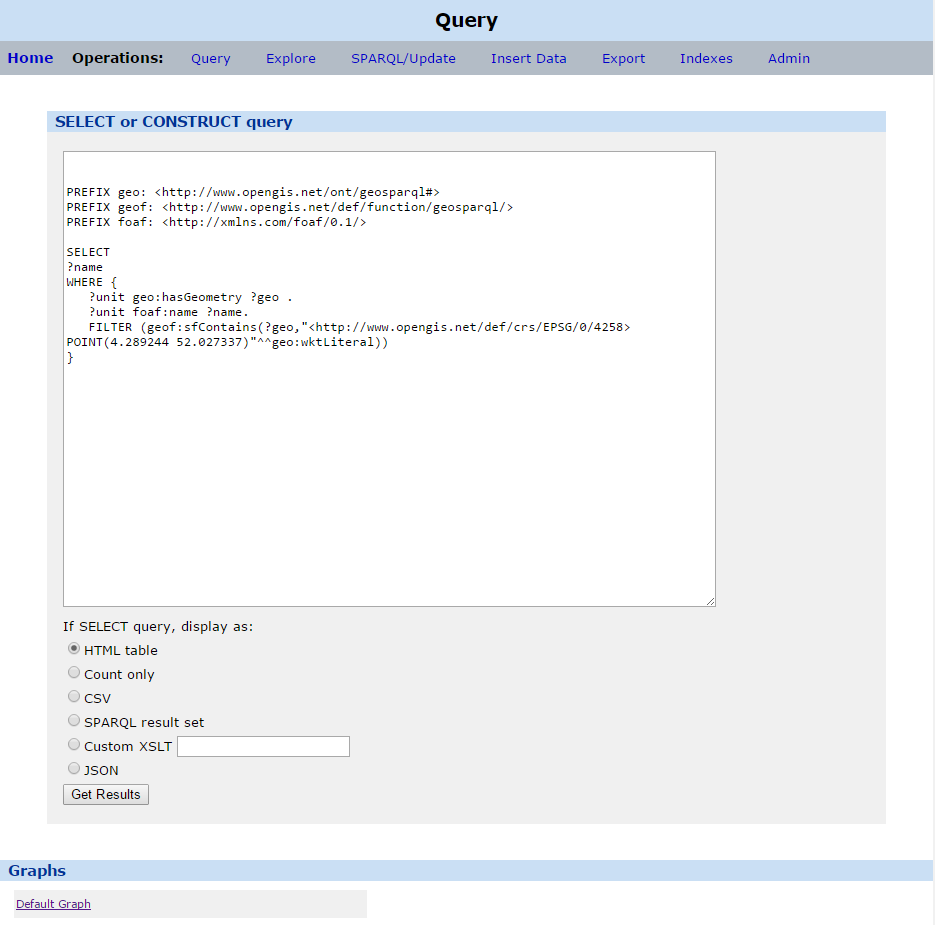
\includegraphics[width=\linewidth]{figs/Parliament.PNG}
	\caption{Parliament endpoint}
	\label{fig:Parliament}
\end{figure}

%\begin{figure}
	%\centering
%	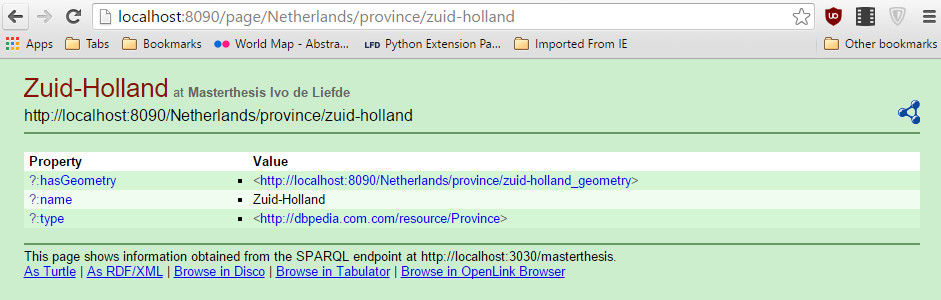
\includegraphics[width=\linewidth]{figs/pubby.PNG}
%	\caption{Pubby interface for \ac{rdf}}
%	\label{fig:Pubby}
%\end{figure}


\section{Retrieving metadata from the Sensor Observation Service}
The metadata is automatically retrieved from the \ac{sos}.

A sequence of request are being made to retrieve all the desired data: observed properties, procedures, features of interest, locations of features of interest, procedures related to features of interest, observed properties related to procedures and metadata about the \ac{sos} (name, organisation, requests, filters and formats it supports).

%problems: 
%\begin{itemize}
%	\item Observation are the central concept in a \ac{sos}. This makes it hard to retrieve the locations of the sensors from the capabilities document. A workaround is to retrieve small amounts of observations for each feature of interest.
%	\item Although standardised, the \ac{sos} contains information that can be implemented in different ways. This makes it hard to automatically retrieve data. An example is the feature of interest in the \texttt{GetObservation} document. 
%\end{itemize}

\section{Modelling with the om-lite and sam-lite ontologies}
Using the ontologies to create a model that suits the purpose of this thesis.

\section{Establishing inward links from DBPedia}
Sending triples to DBPedia the project.

\section{Setting up the Web Processing Services}
Creating two \ac{wps} using PyWPS.

\section{Prototype implementation}
Crawling the semantic web to find specific sensor data.